% Created 2020-04-14 Tue 21:18
% Intended LaTeX compiler: pdflatex
\documentclass[11pt]{article}
\usepackage[utf8]{inputenc}
\usepackage[T1]{fontenc}
\usepackage{graphicx}
\usepackage{grffile}
\usepackage{longtable}
\usepackage{wrapfig}
\usepackage{rotating}
\usepackage[normalem]{ulem}
\usepackage{amsmath}
\usepackage{textcomp}
\usepackage{amssymb}
\usepackage{capt-of}
\usepackage{hyperref}
\usepackage{minted}
\usepackage{amsmath}
\usepackage{esint}
\usepackage[english, russian]{babel}
\usepackage{mathtools}
\usepackage{amsthm}
\usepackage[top=0.8in, bottom=0.75in, left=0.625in, right=0.625in]{geometry}
\author{Sergey Makarov}
\date{\today}
\title{}
\hypersetup{
 pdfauthor={Sergey Makarov},
 pdftitle={},
 pdfkeywords={},
 pdfsubject={},
 pdfcreator={Emacs 26.3 (Org mode 9.3)}, 
 pdflang={Russian}}
\begin{document}


\section{Задача 1}
\label{sec:orgb8491eb}
Построить магазинный автомат для языка \(L_=\).
\subsection{Решение}
\label{sec:orga307f05}
\(L_=\) -- язык слов, в которых количество букв \(a\) и \(b\) одинаково. Чтобы смоделировать этот
язык, будем поддерживать инвариант: количество букв \(a\) и \(b\) в слове, образованном уже
прочитанной частью входного слова, сконкатенированной с содержимым стека, должно быть
одинаковым. Этот инвариант приводит нас к следующей схеме:
\begin{equation}
P = (Q, \Sigma, \Gamma, \delta, q_0, Z_0, F),
\end{equation}
где
\begin{equation}
\begin{cases}
Q = \{q_0, q_1, q_2\}, \\
\Sigma = \{a, b\}, \\
\Gamma = \{a, b, \$\}, \\
q_0 = q_0, \\
Z_0 = \$, \\
F = \{q_0\}.
\end{cases}
\end{equation}
Здесь состояния имеют смысл:
\begin{enumerate}
\item $q_0$ -- количество букв $a$ и $b$ в прочитанной части слова одинаково.
\item $q_1$ -- букв $a$ в прочитанной части слова больше, чем букв $b$.
\item $q_2$ -- букв $b$ в прочитанной части слова больше, чем букв $a$.
\end{enumerate}
Распишем функцию переходов:
\begin{equation}
\begin{cases}
\delta(q_0, a, \$) = (q_1, b\$), \\
\delta(q_0, b, \$) = (q_2, a\$), \\
\delta(q_1, a, b) = (q_1, bb), \\
\delta(q_1, b, b) = (q_1, \varepsilon), \\
\delta(q_1, \varepsilon, \$) = (q_0, \$), \\
\delta(q_2, a, a) = (q_2, \varepsilon), \\
\delta(q_2, b, a) = (q_2, aa), \\
\delta(q_2, \varepsilon, \$) = (q_0, \$)
\end{cases}
\end{equation}
Все переходы, не обозначенные здесь, ведут в dead state, сигнализирующее об ошибке.
Изобразим этот автомат в виде диаграммы переходов(dead state опущено):
\begin{center}
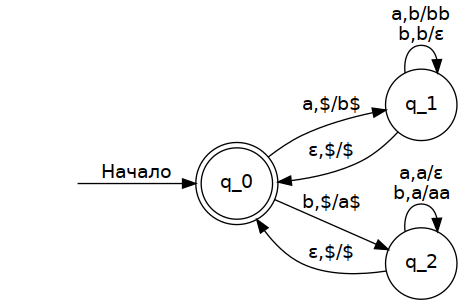
\includegraphics[height=150px]{diag1.png}
\end{center}
\section{Задача 4}
\label{sec:org629bba3}
Построить магазинный автомат для языка \(D_1\).
\subsection{Решение}
\label{sec:org4001261}
Для данной задачи удобнее использовать автомат, допускающий строку по пустому магазину. В
основу описания автомата положен следующий алгоритм распознавания ПСП:
\begin{enumerate}
\item Распознавание начинается с пустым стеком, символы читаются по одному.
\item Если встречена открывающая скобка, она кладётся в стек и происходит переход к следующему символу.
\item Если встречена закрывающая скобка, со стека снимается последняя открывающая скобка. Если стек был пуст, строка не является ПСП.
\item Если после прочтения всей строки стек пуст, строка является корректной ПСП, в противном случае нет.
\end{enumerate}
Этот алгоритм приводит к следующему автомату:
\begin{equation}
P = (Q, \Sigma, \Gamma, \delta, q_0, Z_0, F), где
\end{equation}
\begin{equation}
\begin{cases}
Q = \{q_0, q_1\}, \\
\Sigma = \{ (, )\}, \\
\Gamma = \{(, \$\}, \\
q_0 = q_0, \\
Z_0 = \$, \\
F = \{q_1\}, \\
\delta(q_0, (, \$) = (q_0, (\$), \\
\delta(q_0, (, () = (q_0, ((), \\
\delta(q_0, ), () = (q_0, \varepsilon), \\
\delta(q_0, \varepsilon, \$) = (q_1, \$).
\end{cases}
\end{equation}
Или, если изображать графически:
\begin{center}
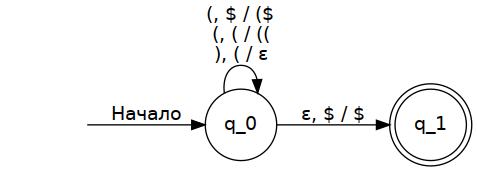
\includegraphics[height=100px]{diag2.png}
\end{center}
\section{Задача 6}
\label{sec:org75f7eee}
Построить детерминированный магазинный автомат для языка \(\{a^nb^mc^n | m, n \geq 0\}\).
\subsection{Решение}
\label{sec:org47397be}
Будем использовать три состояния:
\begin{enumerate}
\item Состояние {}<<чтения префикса из a>>{}. В этом состоянии автомат читаем символы a и кладёт их на стек.
\item Состояние {}<<чтения средней части слова>>{}. В этом состоянии автомат пропускает символы b. При реализации это состояние разделяется на два, поскольку, когда стек пустой, это состояние является завершающим, а когда стек непуст -- не является.
\item Состояние {}<<чтения суффикса из c>>{}. В этом состоянии автомат читает символы c и снимает символы a со стека. Если ввод и стек исчерпались не одновременно, строка некорректна.
\end{enumerate}
Получаем автомат:
\begin{equation}
P = (Q, \Sigma, \Gamma, \delta, q_0, Z_0, F),
\end{equation}
где
\begin{equation}
\begin{cases}
Q = \{q_0, q_1, q_2, q_3, q_4, q_5\}, \\
\Sigma = \{a, b, c\}, \\
\Gamma = \{a, \$\}, \\
q_0 = q_0, \\
Z_0 = \$, \\
F = \{q_0, q_1, q_5\}.
\end{cases}
\end{equation}
Функция переходов:
\begin{equation}
\begin{cases}
\delta(q_0, a, \$) = (q_2, a\$), \\
\delta(q_0, b, \$) = (q_1, \$), \\
\delta(q_1, b, \$) = (q_1, \$), \\
\delta(q_2, a, a)  = (q_2, aa), \\
\delta(q_2, b, a)  = (q_3, a), \\
\delta(q_2, c, a)  = (q_4, \varepsilon), \\
\delta(q_3, b, a)  = (q_3, a), \\
\delta(q_3, c, a)  = (q_3, \varepsilon), \\
\delta(q_4, c, a)  = (q_4, \varepsilon), \\
\delta(q_4, \varepsilon, \$) = (q_5, \varepsilon).
\end{cases}
\end{equation}
Или, в виде диаграммы состояний:
\begin{center}
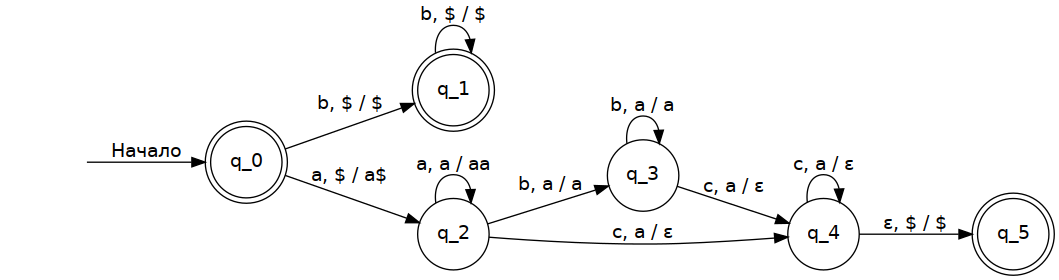
\includegraphics[height=100px]{diag3.png}
\end{center}

Как и в прошлых задачах, переходы в dead state опущены.
\section{Задача 7}
\label{sec:orgd9e22b2}
Построить магазинный автомат по описанию грамматики:
\begin{equation}
\begin{cases}
S \rightarrow AB \\
A \rightarrow aA | \varepsilon \\
B \rightarrow bB | \varepsilon \\
\end{cases}
\end{equation}
\subsection{Решение}
\label{sec:org3ea388c}
Язык данной грамматики может быть разобран методом рекурсивного спуска следующим образом:
\begin{minted}[]{c}
char look;

void parseS() {
    parseA();
    parseB();
}

void parseA() {
    if ((look = getchar()) == 'a') {
        parseA();
    }
}

void parseB() {
    if ((look = getchar()) == 'b') {
        parseB();
    }
}
\end{minted}
Смоделируем работу рекурсивного спуска с помощью магазинного автомата:
\begin{equation}
P = (Q, \Sigma, \Gamma, \delta, q_0, Z_0, F),
\end{equation}
где
\begin{equation}
\begin{cases}
Q = \{q_0, q_1, q_2\}, \\
\Sigma = \{a, b\}, \\
\Gamma = \{a, b, A, B, \$\}, \\
q_0 = q_0, \\
Z_0 = \$, \\
F = \{q_0, q_1, q_2\}
\end{cases}
\end{equation}
Таблица переходов:
\begin{equation}
\begin{cases}
\delta(q_0, \varepsilon, \$) = (q_0, S\$), \\
\delta(q_0, \varepsilon, S) = (q_0, AB), \\
\delta(q_0, a, A) = (q_1, A), \\
\delta(q_0, b, A) = (q_2, \varepsilon), \\
\delta(q_1, a, A) = (q_1, A), \\
\delta(q_1, b, A) = (q_2, \varepsilon), \\
\delta(q_2, b, B) = (q_2, B).
\end{cases}
\end{equation}
Или, в виде диаграммы:
\begin{center}
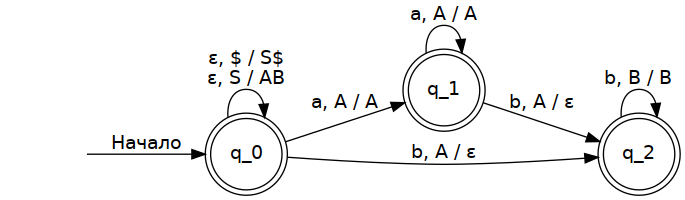
\includegraphics[height=100px]{diag4.png}
\end{center}
\section{Задача 11}
\label{sec:org94191c7}
Привести грамматику к нормальной форме Хомского:
\begin{equation}
\begin{cases}
S \rightarrow A | C, \\
A \rightarrow aAB, \\
C \rightarrow CB | C, \\
A \rightarrow \varepsilon, \\
B \rightarrow b.
\end{cases}
\end{equation}
\subsection{Решение}
\label{sec:org96af275}
В грамматике присутствует \(\varepsilon\)-продукция \(A \rightarrow \varepsilon\). Удаление этой
продукции приводит к грамматике:
\begin{equation}
\begin{cases}
S \rightarrow A | C, \\
A \rightarrow aAB | aB, \\
C \rightarrow CB | C, \\
B \rightarrow b.
\end{cases}
\end{equation}

В получившейся грамматике нет \(\varepsilon\)-продукций, но есть цепные продукции \(S \rightarrow A\),
\(S \rightarrow C\) и \(C \rightarrow C\). Удаление этих продукций приводит к грамматике:
\begin{equation}
\begin{cases}
S \rightarrow aAB | aB | CB, \\
A \rightarrow aAB | aB, \\
C \rightarrow CB, \\
B \rightarrow b.
\end{cases}
\end{equation}

В получившейся грамматике нет \(\varepsilon\)-продукций и цепных продукций, но есть бесполезные
символы, в частности, символ \(C\), не порождающий ни одной строки из терминальных символов.
Удаление этого символа приводит к грамматике:
\begin{equation}
\begin{cases}
S \rightarrow aAB | aB, \\
A \rightarrow aAB | aB, \\
B \rightarrow b.
\end{cases}
\end{equation}
Все нетерминалы этой грамматики являются порождающими. В самом деле, нетерминал \(S\) порождает
например строку \(ab\), нетерминал \(A\) порождает ту же строку \(ab\), нетерминал \(B\) порождает
строку \(B\). Недостижимых символов в этой грамматике так же нет, символы \(a, A\) и \(B\) достижимы
непосредственно из \(S\), символ \(b\) достижим из \(B\).

В полученной грамматике уже нет ни бесполезных символов, ни \(\varepsilon\)-продукций, ни цепных
продукций, но это всё ещё не нормальная форма Хомского, так как в ней все правила должны иметь
вид либо \(A \rightarrow BC\), либо \(B \rightarrow b\). Грамматика (16) приводится к такому виду
путём введения дополнительных символов:
\begin{equation}
\begin{cases}
S   \rightarrow A'B | A''B, \\
A'  \rightarrow a, \\
A'' \rightarrow A'A, \\
A   \rightarrow A'B | A''B, \\
B   \rightarrow b.
\end{cases}
\end{equation}
Заметим, что полученная грамматика не эквивалентна исходной грамматике (13): в отличие от неё
эта грамматика не допускает пустую цепочку. Эта проблема решается добавлением \(\varepsilon\)-правила
\(S \rightarrow \varepsilon\), но полученная грамматика уже не будет находиться в кормальной форме
Хомского.
\section{Задача 16}
\label{sec:org71a0505}
Показать, что язык \(L = \{b^p | p\text{ -- простое}\}\) не является контекстно-свободным.
\subsection{Решение}
\label{sec:org5877656}
Пусть данный язык является контекстно-свободным. По лемме о накачке для контекстно-свободных
языков \(\exists n: \forall z \in L |z| \geq n: z = uvwxy\), причём:
\begin{enumerate}
\item \(|vwx| \leq n\).
\item \(vx \neq \varepsilon\).
\item \(uv^iwx^iy \in L \forall i \geq 0\).
\end{enumerate}
Пусть \(z = b^p\), где \(p\) - минимальное простое число, не меньшее \(n\). Обозначим
\(|u| + |w| + |y| = p, |v| + |x| = q\). Из условий леммы о накачке \(b^{p + qi} \in L \forall i \geq 0\).
Получаем противоречие с тем, что цепочка \(b^{p + qp} = b^{(q + 1)p}\) не может принадлежать языку,
так как число \((q + 1)p\) не является простым, поскольку делится на \((q + 1) > 1\).
\section{Задача 17}
\label{sec:org4add8c8}
Показать, что язык \(\{uu | u \in \Sigma^*\}\) не является контекстно-свободным.
\subsection{Решение}
\label{sec:orgd43007c}
Пусть данный язык является контекстно-свободным. По лемме о накачке для контекстно-свободных
языков \(\exists n: \forall z \in L |z| \geq n: z = uvwxy\), причём:
\begin{enumerate}
\item \(|vwx| \leq n\).
\item \(vx \neq \varepsilon\).
\item \(uv^iwx^iy \in L \forall i \geq 0\).
\end{enumerate}
Пусть \(z = a^nb^na^nb^n\). Возможны два случая:
\begin{itemize}
\item В цепочке \(vx\) количество букв \(a\) и \(b\) разное. Тогда накачивая \(v\) и \(x\) можно получить цепочку, в которой разность количества букв \(a\) и \(b\) будет сколь угодно большой. Но в любом слове языка \(L\) количество букв \(a\) и \(b\) должно быть одинаковым, так что полученное слово не может принадлежать \(L\).
\item В цепочке \(vx\) количество букв \(a\) и \(b\) одинаковое. Это означает, что цепочка \(vwx\) захватывает часть одного из блоков букв \(a\) и часть соседнего блока букв \(b\)(остальные случаи невозможны, поскольку длина всей цепочки меньше длины блока). Здесь также возможны два случая:
\begin{itemize}
\item Цепочка \(vwx\) располагается в одном из блоков \(a^nb^n\). Разобьём цепочку \(z\) на два блока \(a^nb^n\). Тогда при накачивании будет увеличиваться один из этих блоков, а второй изменяться не будет. Рассмотрим строчку \(uwy\). По условию эта строка тоже должна принадлежать \(L\). С другой стороны, строка \(uwy\) получается путём конкатенации блока \(a^kb^k, 0 < k < n\) и блока \(a^nb^n\). Если {}<<короткий>>{} блок идёт до {}<<длинного>>{}, эта строчка не может принадлежать \(L\), поскольку первая половина строки заканчивается на \(a\), а вторая -- на \(b\). Если {}<<короткий>>{} блок идёт после {}<<длинного>>{}, эта строка также не принадлежит \(L\), поскольку половины цепочки начинаются с разных букв.
\item Цепочка \(vwx\) располагается в блоке \(b^na^n\). Разобьём цепочку \(z\) на три блока: \(a^n\), \(b^na^n\), \(b^n\). Теперь рассмотрим строку \(uwy\), полученную из \(z\) путём выкидывания частей \(v\) и \(x\). На первую и третью части эта операция не повлияет. Вторая часть же примет вид \(b^ka^k, 0 < k < n\)(из строки \(b^na^n\) удалили две подстроки, в которых суммарно одинаковое количество букв \(a\) и \(b\), поэтому ничего другого получиться не могло). Получаем цепочку вида \(a^nb^ka^kb^n\), половины которой \(a^nb^k\) и \(a^kb^n\), как легко видеть, не совпадают.
\end{itemize}
\end{itemize}
Итак, получаем, что либо {}<<расширенная>>{} цепочка, либо цепочка \(uwy\) не принадлежит \(L\), что противоречит лемме о накачке при условии, что \(L\) -- КС-язык. Таким образом, язык \(L\) не является контекстно-свободным, что и требовалось доказать.
\end{document}
